\chapter{Data Foundation}
\label{data}
In this chapter the provided datasets from the previously mentioned street information systems and the FCD provider will be elaborated. First an overview of FCD in general and the available dataset is given. To give an overview about what results can be expected the incident datasets from BAYSIS and ArbIS are presented with descriptive statistic. The most relevant parameters of the datasets will be elaborated and illustrated. The parameters are also categorized in the variable types, defined in chapter \autoref{correlation_variable_types}.

\section{Floating-Car-Data (FCD)}
\label{dataset_fcd}
 
As described in chapter 1.1, \acrshort{fcd} represents the movement of vehicles and can be used to calculate vehicle speeds and trajectories. The provided dataset contains the aggregated absolute and relative speeds for the highways and state streets, calculated from \acrshort{fcd} data. The process of speeds estimation with \acrshort{fcd} data is explained in detail by Felix Rampe in chapter 4 of his thesis \textit{Traffic Speed Estimation and Prediction Using Floating Car Data} \parencite{Rempe2018}, but is outside of the scope for this thesis. The FCD is mapped onto the HERE \parencite{HERE2020} network, to be compliant with the geolocation system used in the project.

% TODO add more info about FCD if there is time 
% https://athene-forschung.unibw.de/doc/127445/127445.pdf
% Traffic Speed Estimation and Prediction Using Floating Car Data.pdf

Each of these aggregated speeds now represents the mean speed over a three minute time interval on the corresponding road section. This arrangement of speeds for each time step and space step is called speed matrix and is the base data for the congestion detection. Figure \autoref{img:speedMatrixPlot_mutipleMixedClusters} shows a visual representation a speed matrixes with the horizontal axes being the spatial extend and the vertical axes the time extend. Deep greens represent free flowing traffic with ~130 km/h, which is the norm speed in Germany (in German called “Richtgeschwindigkeit”) on highways set the legislator. The speed scale then develops linearly downwards deep red indicating traffic with 30 km/h or less. 

\begin{figure}[ht]
	\centering
	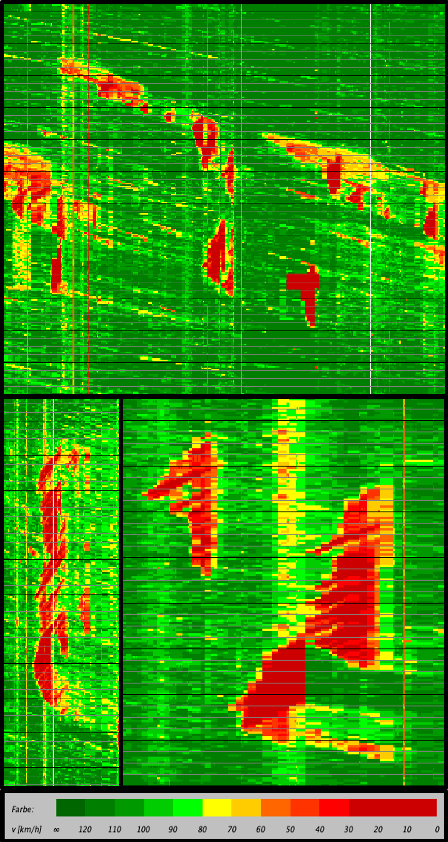
\includegraphics[scale=0.7]{images/SpeedMatrixPlot_mutiple}
	\caption{Speed matrix plots of processed FCD data, showing different jam clusters}
	\label{img:speedMatrixPlot_mutipleMixedClusters}
\end{figure}

The observer will clearly recognize the jams represented by the clusters of red and orange cells in the figure \autoref{img:speedMatrixPlot_mutipleMixedClusters}, with the angled extends towards the right down edge, due to the vehicle trajectory through space and time. These cluster, also shown in the two lower pictures, which representing one or multiple jams can be densely packed or spotted into smaller clusters or, depending on the severity of a jam can be seen, by the cluster which contain more orange or yellow cells than red. 

From this visual clarity, the continuity of the data points and the precision on 3-minute intervals it can concluded that a comprehensive algorithmic approach should be able to detect such congestion events. This being said, the dataset does contain defects in the form of missing values for complete road sections, which can interfere with detection algorithm. Another defect type are obviously wrong speed block, meaning sudden speed drops or jumps to areas of identical speeds with an abnormal temporal and spatial extend, which have to be ignored during processing. 

\section{Accident Data (BAYSIS)}
\label{dataset_baysis}

The \acrfull{baysis} as describe in chapter \autoref{dataset_baysis}, collects a wide range of different information types, one of then being accidents with the corresponding police reports. The provided export from BAYSIS contains all accidents of the year 2019 on the Bavarian highway network, which are 10262 records in number. 

Each accident report includes a variety of specifications, which covers environmental indicators like weather or light situation, accident characteristics like accident type, collision object or cause, as well as information over the involved like nationality, age and gender. In total, one report contains 132 values, describing the accident, participant and environment. Because we do not want to form a stereotype of accident participant but rather find significant accident characteristics or environmental factors most of the descriptive values for the involved persons are not considered. Variables without any values or single values are also neglected. To meet a statistical significant result a diverse distribution in the values would be preferred, to reduce the risk of uncertain relation. Because the correlation of a non distributed variable, which for example has one values occupying a 95\% major share, is based on a sample set comprised of mostly the same samples, the interpretability for a correlation to other values but the major share is very limited (see \autoref{correlation_significance_uncertainty} for more detailed elaboration of this assumption).

From this curtailed pool of correlate able and analyze able characteristics all parameters that have a logical significance with causes or effects of an accident will be considered in the analysis.  The referred figures are available as larger prints in the appendix \autoref{appendix_baysis} for better readability, as they do not properly fit in the text. 

\begin{figure}[ht]
	\centering
	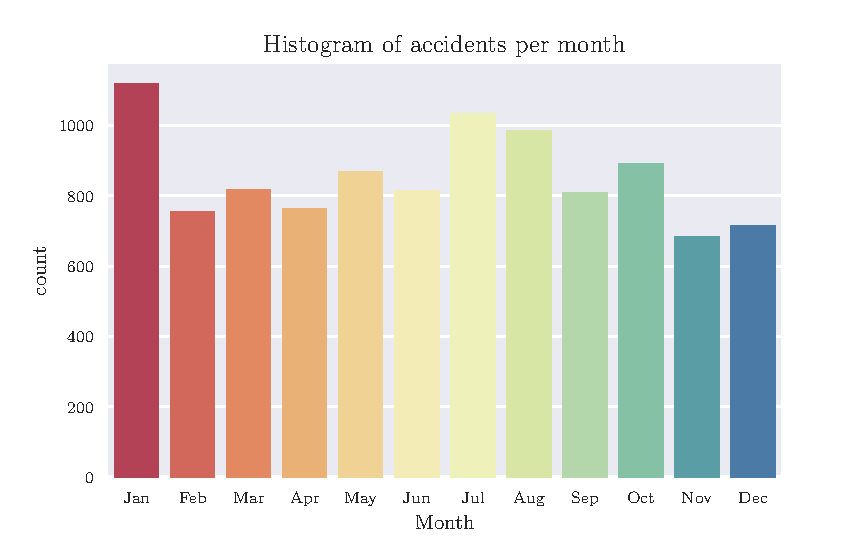
\includegraphics[scale=0.9]{CorrAnalysis/data/BAYSIS/01_dataset/plots/baysis_dataset_hist_month}
	\caption{Monthly distribution of accident counts}
	\label{img:baysis_dataset_dist_month}
\end{figure}

A look on the monthly distribution of accidents recorded by BAYSIS (see figure \autoref{img:baysis_dataset_dist_month}) shows that that the months of January, July and August have considerably higher number of accidents, with respectively 31\,\%, 21\,\% and 15\,\% increase over the mean count of 855 accidents per month. The increased number in January can be explained with the increased number of accidents due to ice and snow conditions, which reduces traction on roads and can lead to uncontrollable vehicle behavior. Also the reduced visibility during snow falls increases accident numbers. In July and August the increased traffic volume because of public holidays is the most probable explanation for the higher number of accidents. 

Another valuable distribution is the number of accidents per road (see figure \autoref{img:baysis_dataset_dist_highway}). The roads A3, A9 and A8 have relative high count of accidents. In contrast the road A71 and downwards have only an accidents and therefore have a high uncertainty associated with them. 

\clearpage

\begin{figure}[ht]
	\centering
	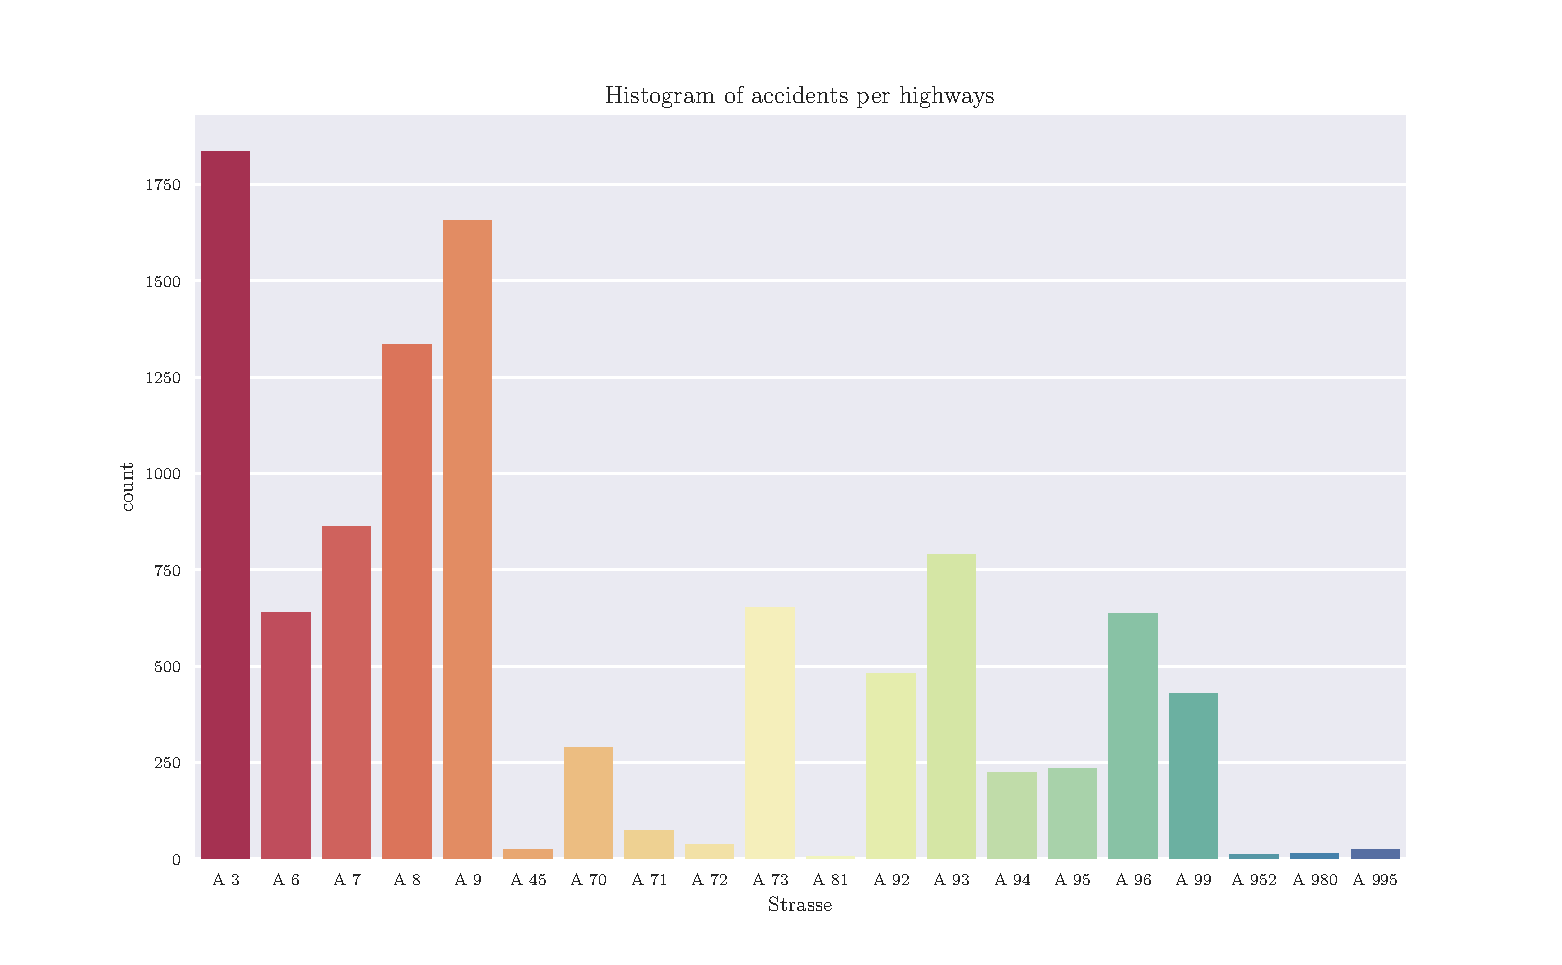
\includegraphics[scale=0.75]{CorrAnalysis/data/BAYSIS/01_dataset/plots/baysis_dataset_hist_highway}
	\caption{Distribution of accident counts, by road}
	\label{img:baysis_dataset_dist_highway}
	\vspace{-8mm}
\end{figure}

\paragraph{Kat}
The accident category (shown table \autoref{tbl:baysis_dataset_Kat} and visualized figure \autoref{img:appendix_baysis_dataset_Kat}), describes the which damages or injuries can be associated with the accident. It ranges from accident with just  damaged property, lightly and heavily injured to deathly accidents. The distribution develops from lowest to highs counts, in order of gravity of the category. The variable consists of four values, which can be ordered, and is therefore ordinal.
\begin{table}[!ht]
	\centering
	\small
	\begin{tabular}{c|c|c|l} 
		\toprule
		Code & Count & Freq. [\%] & Description \\ 
		\midrule
 		0 	& - 	& 	-	& Minor Accident  \\
 		1 	& 76 	& 0.7 	& Accident with deaths  \\ 
 		2 	& 600	& 5.8	& Accident with heavily injured  \\
 		3 	& 2685	& 26.2	& Accident with lightly injured  \\
		7 	& 6900	& 67.2	& Accident with property damage  \\
		\bottomrule
	\end{tabular}
	\caption{Descriptive of \textbf{Kat}}
	\label{tbl:baysis_dataset_Kat}
	\vspace{-8mm}
\end{table}

\paragraph{Typ}
The accident type variable (shown table \autoref{tbl:baysis_dataset_Typ} and visualized figure \autoref{img:appendix_baysis_dataset_Typ}) incorporates different kind of traffic movements, from straight driving to turning movements or merging. It describes during which kind of movement the accident happened. Beside of an 80\,\% share of accidents related to driving or straight driving situations, the parameter does not indicate any other features. The variable does not show any order and is therefore of nominal type.
\begin{table}[!ht]
	\centering
	\small
	\begin{tabular}{c|c|c|l} 
		\toprule
		Code & Count & Freq. [\%] & Description \\ 
		\midrule
 		1 & 2820	& 27.5	& Driving accident \\ 
 		2 & 1		& < 0.1 & Turning accident \\
 		3 & 373		& 3.6 	& Merging / Crossing accident \\
 		4 & 10		& 0.1	& Crossing over accident \\
 		5 & 160 	& 1.6	& Accident in standing traffic \\
 		6 & 5285	& 51.5	& Accident in straight traffic \\
		7 & 1612	& 15.7 	& Other \\
		\bottomrule
	\end{tabular}
	\caption{Descriptive of \textbf{Typ}}
	\label{tbl:baysis_dataset_Typ}
	\vspace{-8mm}
\end{table}

\paragraph{Betei}
The distribution of the number of involved persons (shown table \autoref{tbl:baysis_dataset_Betei} and visualized figure \autoref{img:appendix_baysis_dataset_Betei}) shows that more than 96\,\% of accidents have three or less involved persons, supported by a mean of 1.9 involved persons. The major share of two involved persons makes up for 56\,\% and the second biggest of one involved person for 30\,\% of the total count. Because of the increasing order of values, the variable is of ordinal type.
\begin{table}[!ht]
	\centering
	\small
	\begin{tabular}{r|ccccccc} 
		\toprule
		 			& 1		& 2		& 3		& 4		& 5		& 6  	& > 7\\ 
		\midrule
 		Count 		& 2768	& 6047	& 1085	& 235	& 72 	& 24	& 30 \\ 
 		Freq. [\%] 	& 27.0	& 58.9	& 10.6 	& 2.3	& 0.7 	& 0.2 	& 0.1 \\
		\bottomrule
	\end{tabular}
	\caption{Descriptive of \textbf{Betei}}
	\label{tbl:baysis_dataset_Betei}
	\vspace{-8mm}
\end{table}

\paragraph{UArt}
\label{baysis_dataset_UArt}
The accident cause type is defined by the two variables \textbf{UArt1} and \textbf{UArt2} (shown table \autoref{tbl:baysis_dataset_UArt} and visualized figure \autoref{img:appendix_baysis_dataset_UArt}), whereat the first is the more suitable one. They describe the type of collision cause and presents two major sets. One being the accidents with waiting, stopping and starting vehicles in the same lane, which describe typical collision accidents during congested traffic. The other being the accidents in the next left or right lane, which describe common lane changing collisions. Accidents with cross traffic, pedestrians or opposite traffic are relatively uncommon. The variable does not show any order and is therefore of nominal type.
\begin{table}[ht]
	\centering
	\small
	\begin{tabular}{c|c|c|c|l} 
		\toprule
		Code & Count[1] & Count[2] & Freq. [\%] & Description \\ 
		\midrule
 		1 & 466		& 13	& & Collision with starting, standing or stopping vehicle  \\ 
 		2 & 2111	& 44 	& & Collision with ahead and waiting vehicle  \\
 		3 & 2873	& 140	& & Collision with vehicle on separate lane in same direction  \\
 		4 &	16		& 4		& & Collision with vehicle going in opposite direction  \\
 		5 & 240		& 12	& & Collision with turning or crossing vehicle  \\
 		6 & 19		& 1		& & Collision between vehicle and pedestrian  \\
 		7 & 411		& 42	& & Collision with obstacle  \\
 		8 & 1728	& 381	& & Deviation to the right  \\
 		9 & 1446	& 517	& & Deviation to the left  \\
		0 & 951		& 42	& & Other  \\
		\bottomrule
	\end{tabular}
	\caption{Descriptive of \textbf{UArt}}
	\label{tbl:baysis_dataset_UArt}
	\vspace{-8mm}
\end{table}

\paragraph{AUrs}
\label{baysis_dataset_AUrs}
The summarized distribution of the parameters \textbf{AUrs1} and \textbf{AUrs2} (shown table \autoref{tbl:baysis_dataset_AUrs} and visualized figure \autoref{img:appendix_baysis_dataset_AUrs}) shows that the variable is no much distributed and only a small number of categories hold have a relevant sample size. Because of that any correlation to this parameter needs to interpreted with caution, due the the high uncertainty. The variable is of nominal type.
\begin{table}[ht]
	\centering
	\small
	\begin{tabular}{c|c|c|c|l}
		\toprule
		Code & Count[1] & Count[2] & Freq. [\%] & Description \\ 
		\midrule
		70 & - 		& -		& & Slippery street due to oil \\
		71 & -		& -		& & Slippery street due to dirt \\
		72 & 618	& -		& & Slippery street due to snow or ice \\
		73 & 855	& 45	& & Slippery street due to rain \\
		74 & -		& -		& & Slippery street due to other objects \\
		75 & 11		& 12	& & Cart track due to rain, snow or ice \\
		76 & 10		& 3		& & Other condition of road \\
		77 & 1		& -		& & Un-regular condition of traffic signs \\
		78 & -		& -		& & Bad lighting of street \\
		79 & -		& -		& & Bad safety on train crossing \\
		80 & 1		& 3		& & Visibility issues due to fog \\
		81 & 4		& 17 	& & Visibility issues due to rain or hail \\
		82 & 24		& -		& & Visibility issues due to sun or glare \\
		83 & 2		& 3		& & Crosswind \\
		84 & 1		& 14	& & Visibility issues due to storm \\
		85 & -		& -		& & Unsafe roadwork \\
		86 & 21		& -		& & Wild animals \\
		87 & 1		& -		& & Other animals \\
		88 & 134	& 4		& & Other obstacles \\
		89 & 97		& 4		& & Other causes \\
		% Count[1] 0 = 8435 / Count[2] 0 = 10156
		\bottomrule
	\end{tabular}
	\caption{Descriptive of \textbf{AUrs}}
	\label{tbl:baysis_dataset_AUrs}
	\vspace{-8mm}
\end{table}

\pagebreak

\paragraph{AufHi}
\label{baysis_dataset_AufHi}
The obstacle collision distribution (shown table \autoref{table:baysis_dataset_AufHi} and visualized figure \autoref{img:appendix_baysis_dataset_AufHi}) reveals that in most collision accidents car hit the guardrails. The other categories are rather uncommon. With 1,5\,\% of accidents without any collision, it can be stated that in most cases a collision is part of an accident. The counts of the remaining categories are insignificant. The variable does not show any order and is therefore of nominal type.
\begin{table}[ht]
	\centering
	\small
	\begin{tabular}{c|c|c|l} 
		\toprule
		Code & Count & Freq. [\%] & Description \\ 
		\midrule 
		0 & 16 		& 0.2	& Single tree \\
		1 & 12 		& 0.1	& Pillar \\
		2 & 5 		& < 0.1	& Abutment \\
		3 & 3041	& 29.6	& Guardrail \\
		4 & 534		& 5.2	& Other object \\
		5 & 144		& 1.4	& No collision \\
		7 & 2		& < 0.1	& Tree line or alley \\
		8 & 26		& 0.3	& Tree group or forest \\
		9 & 52		& 0.5	& Busches \\
		\bottomrule
	\end{tabular}
	\caption{Descriptive of \textbf{AufHi}}
	\label{table:baysis_dataset_AufHi}
	\vspace{-8mm}
\end{table}

\paragraph{Alkoh}
\label{baysis_dataset_Alkoh}
The alcohol involvement indication parameter only contains one variables of $1 = yes$), whereas an empty variable referred to $no$ or $unknown$. It reveals that only 2.2\,\% of accidents have one or more involved persons with measurable blood alcohol. The variable only has two unique values and is therefore dichotomous.

\paragraph{Char}
\label{baysis_dataset_Char}
The variable Char1 and Char2 (shown table \autoref{table:baysis_dataset_Char} and visualized figure \autoref{img:appendix_baysis_dataset_Char_Bes_Lich}) describe the characteristic of the street where the accident happened. Since we are only considering highway, the type of \textit{Crossing}, \textit{Property} and \textit{Roundabout} is expected to be zero. The variable is not ordered and therefore of nominal type.  
\begin{table}[ht]
	\centering
	\small
	\begin{tabular}{c|c|c|c|l}
		\toprule
		Code & Count[1] & Count[2] & Freq. [\%] & Description \\ 
		\midrule
		1 & - 	& -		&	& Crossing \\
	    2 & 42	& -		&	& Entry / Exit \\
	    3 & 1	& -		&	& Property access \\
	    4 & 380	& -		&	& Incline \\
	    5 & 371	& -		&	& Decline \\
	    6 & 404	& 263	&	& Curve \\
		7 & -	& -		&	& Roundabout \\
		\bottomrule
	\end{tabular}
	\caption{Descriptive of \textbf{Char}}
	\label{table:baysis_dataset_Char}
	\vspace{-8mm}
\end{table}

\paragraph{Bes}
\label{baysis_dataset_Bes}
The variables \textbf{Bes1}, \textbf{Bes2} and \textbf{Bes3} further define the street characteristic mentioned above. But they only contain one variable, referring to the category \textit{Roadwork}. The variable itself is therefore not suitable for a correlation analysis, because it is not distributed, but can be used to validate the roadwork matching performance.
% \begin{table}[ht]
% 	\centering
% 	\begin{tabular}{c|l}  
% 		1 & Confusing \\ 
% 		2 & Level crossing \\
% 		3 & Pedestrian crossing \\
% 		4 & Pedestrian passage \\
% 		5 & Bus-stop \\
% 		6 & Roadwork \\
% 		7 & Calm traffic area \\
% 		8 & RAV on street \\
% 		9 & RAV separate \\
% 		0 & RAV obligatory \\
% 	\end{tabular}
% 	\caption{Identifier and description of 'Bes'}
% 	\label{table:baysis_dataset_Bes}
% \end{table}

\paragraph{Lich}
\label{baysis_dataset_Lich}
The light situation parameter (shown table \autoref{table:baysis_dataset_Lich} and visualized figure \autoref{img:appendix_baysis_dataset_Lich}) describes the lighting condition at the time of the accident. Because it can be ranked from best to worst lighting, both are of ordinal type.
\begin{table}[ht]
	\centering
	\small
	\begin{tabular}{c|c|c|c|l}
		\toprule
		Code & \textbf{Lich1} & \textbf{Lich2} & Freq. [\%] & Description \\ 
		\midrule 
		0 & 6833 	& - 	& & Daylight \\
		1 & 627 	& -		& & Noon \\
		2 & 2560	& - 	& & Darkness \\
		3 & - 		& 3005	& & Street lighting working \\
		4 & - 		& 182	& & Street lighting not working \\
		\bottomrule
	\end{tabular}
	\caption{Descriptive of \textbf{Lich}}
	\label{table:baysis_dataset_Lich}
	\vspace{-8mm}
\end{table} 

\paragraph{Zust}
\label{baysis_dataset_Zust}
The road condition parameter (shown table \autoref{table:baysis_dataset_Zust} and visualized figure \autoref{img:appendix_baysis_dataset_Zust}) describes in which condition the road was at time of the accident in the for of wet, dry, iced or slippery.
\begin{table}[ht]
	\centering
	\small
	\begin{tabular}{c|c|c|c|l}
		\toprule
		Code & \textbf{Zust} & Count[2] & Freq. [\%] & Description \\ 
		\midrule 
		0 & 6851 	& -		& & Dry \\ 
 		1 & 2606	& -		& & Wet \\ 
 		2 & 582		& 207	& & Ice \\
 		3 & - 		& -		& & Slippery (oil, dirt, ...)  \\
	\end{tabular}
	\caption{Descriptive of \textbf{Zust}}
	\label{table:baysis_dataset_Zust}
	\vspace{-8mm}
\end{table}

\paragraph{Fstf}
\label{baysis_dataset_Fstf}
The variable references the lane on which the accident happened (shown table \autoref{table:baysis_dataset_Fstf} and visualized figure \autoref{img:appendix_baysis_dataset_Fstf}). It names the number of lane from the right, the hard-shoulder or the wrong usage of a one-way street. It does not show an order of lanes, but not with the two other types of hard-shoulder and one-way street. It is therefore considered as nominal.
\begin{table}[ht]
	\centering
	\small
	\begin{tabular}{c|c|c|l}
		\toprule
		Code & \textbf{Fstf} & Freq. [\%] & Description \\ 
		\midrule  
		1 & 2821 	& 27.5 	& first lane from the right \\
		2 & 4274 	& 41.7 	& second lane from the right \\
		3 & 1582 	& 15.4 	& third lane from the right \\
		4 & 150 	& 1.5 	& fourth lane from the right \\
		5 & 26 		& 0.3 	& firth lane from the right \\ 
 		S & 247 	& 2.4 	& accident happened on the hard-shoulder lane \\ 
		F & 7 		& 0.1 	& accident happened on opened hard-shoulder lane \\
		\bottomrule
	\end{tabular}
	\caption{Descriptive of \textbf{Fstf}}
	\label{table:baysis_dataset_Fstf}
	\vspace{-8mm}
\end{table}
    
\paragraph{WoTag}
\label{baysis_dataset_WoTag}
The variable of WoTag relates to the day of week, when the accident happened (shown in \autoref{img:baysis_dataset_WoTag}). It is debatable if week days can be ordered, but for this analysis we will consider the parameter of nominal type.
\begin{figure}[ht]
	\centering
	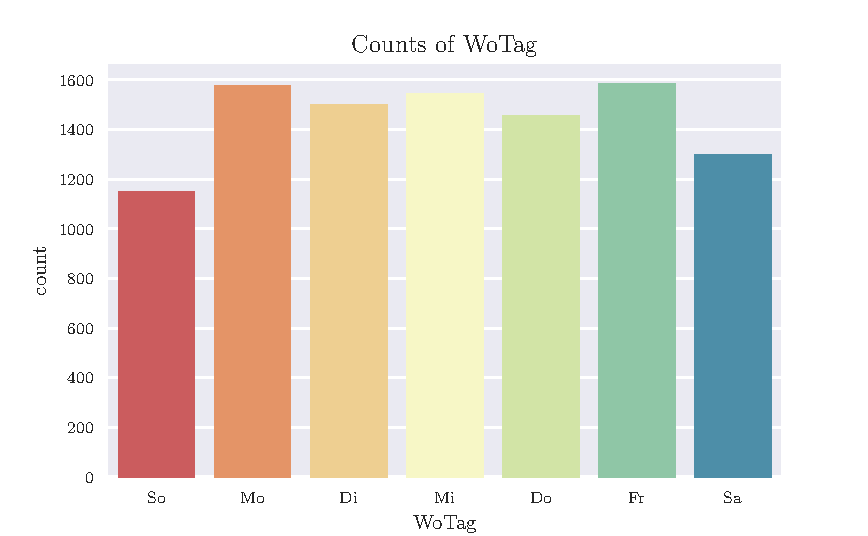
\includegraphics[scale=0.75]{CorrAnalysis/data/BAYSIS/01_dataset/plots/baysis_dataset_count_WoTag}
	\caption{Distribution of accident counts, by week day}
	\label{img:baysis_dataset_WoTag}
	\vspace{-8mm}
\end{figure}

\paragraph{FeiTag}
\label{baysis_dataset_FeiTag}
Only 157 accidents took place on a public holiday. This is not a feature itself but the a possible correlation to jams could be that they are longer because of the increased traffic demand on holidays.
	
% ------- BAYSIS Dataset - Matrix --------
% \newgeometry{left=1.5cm,right=1cm}
% \pagestyle{empty}
% \begin{figure}[ht]
% 	\centering
% 	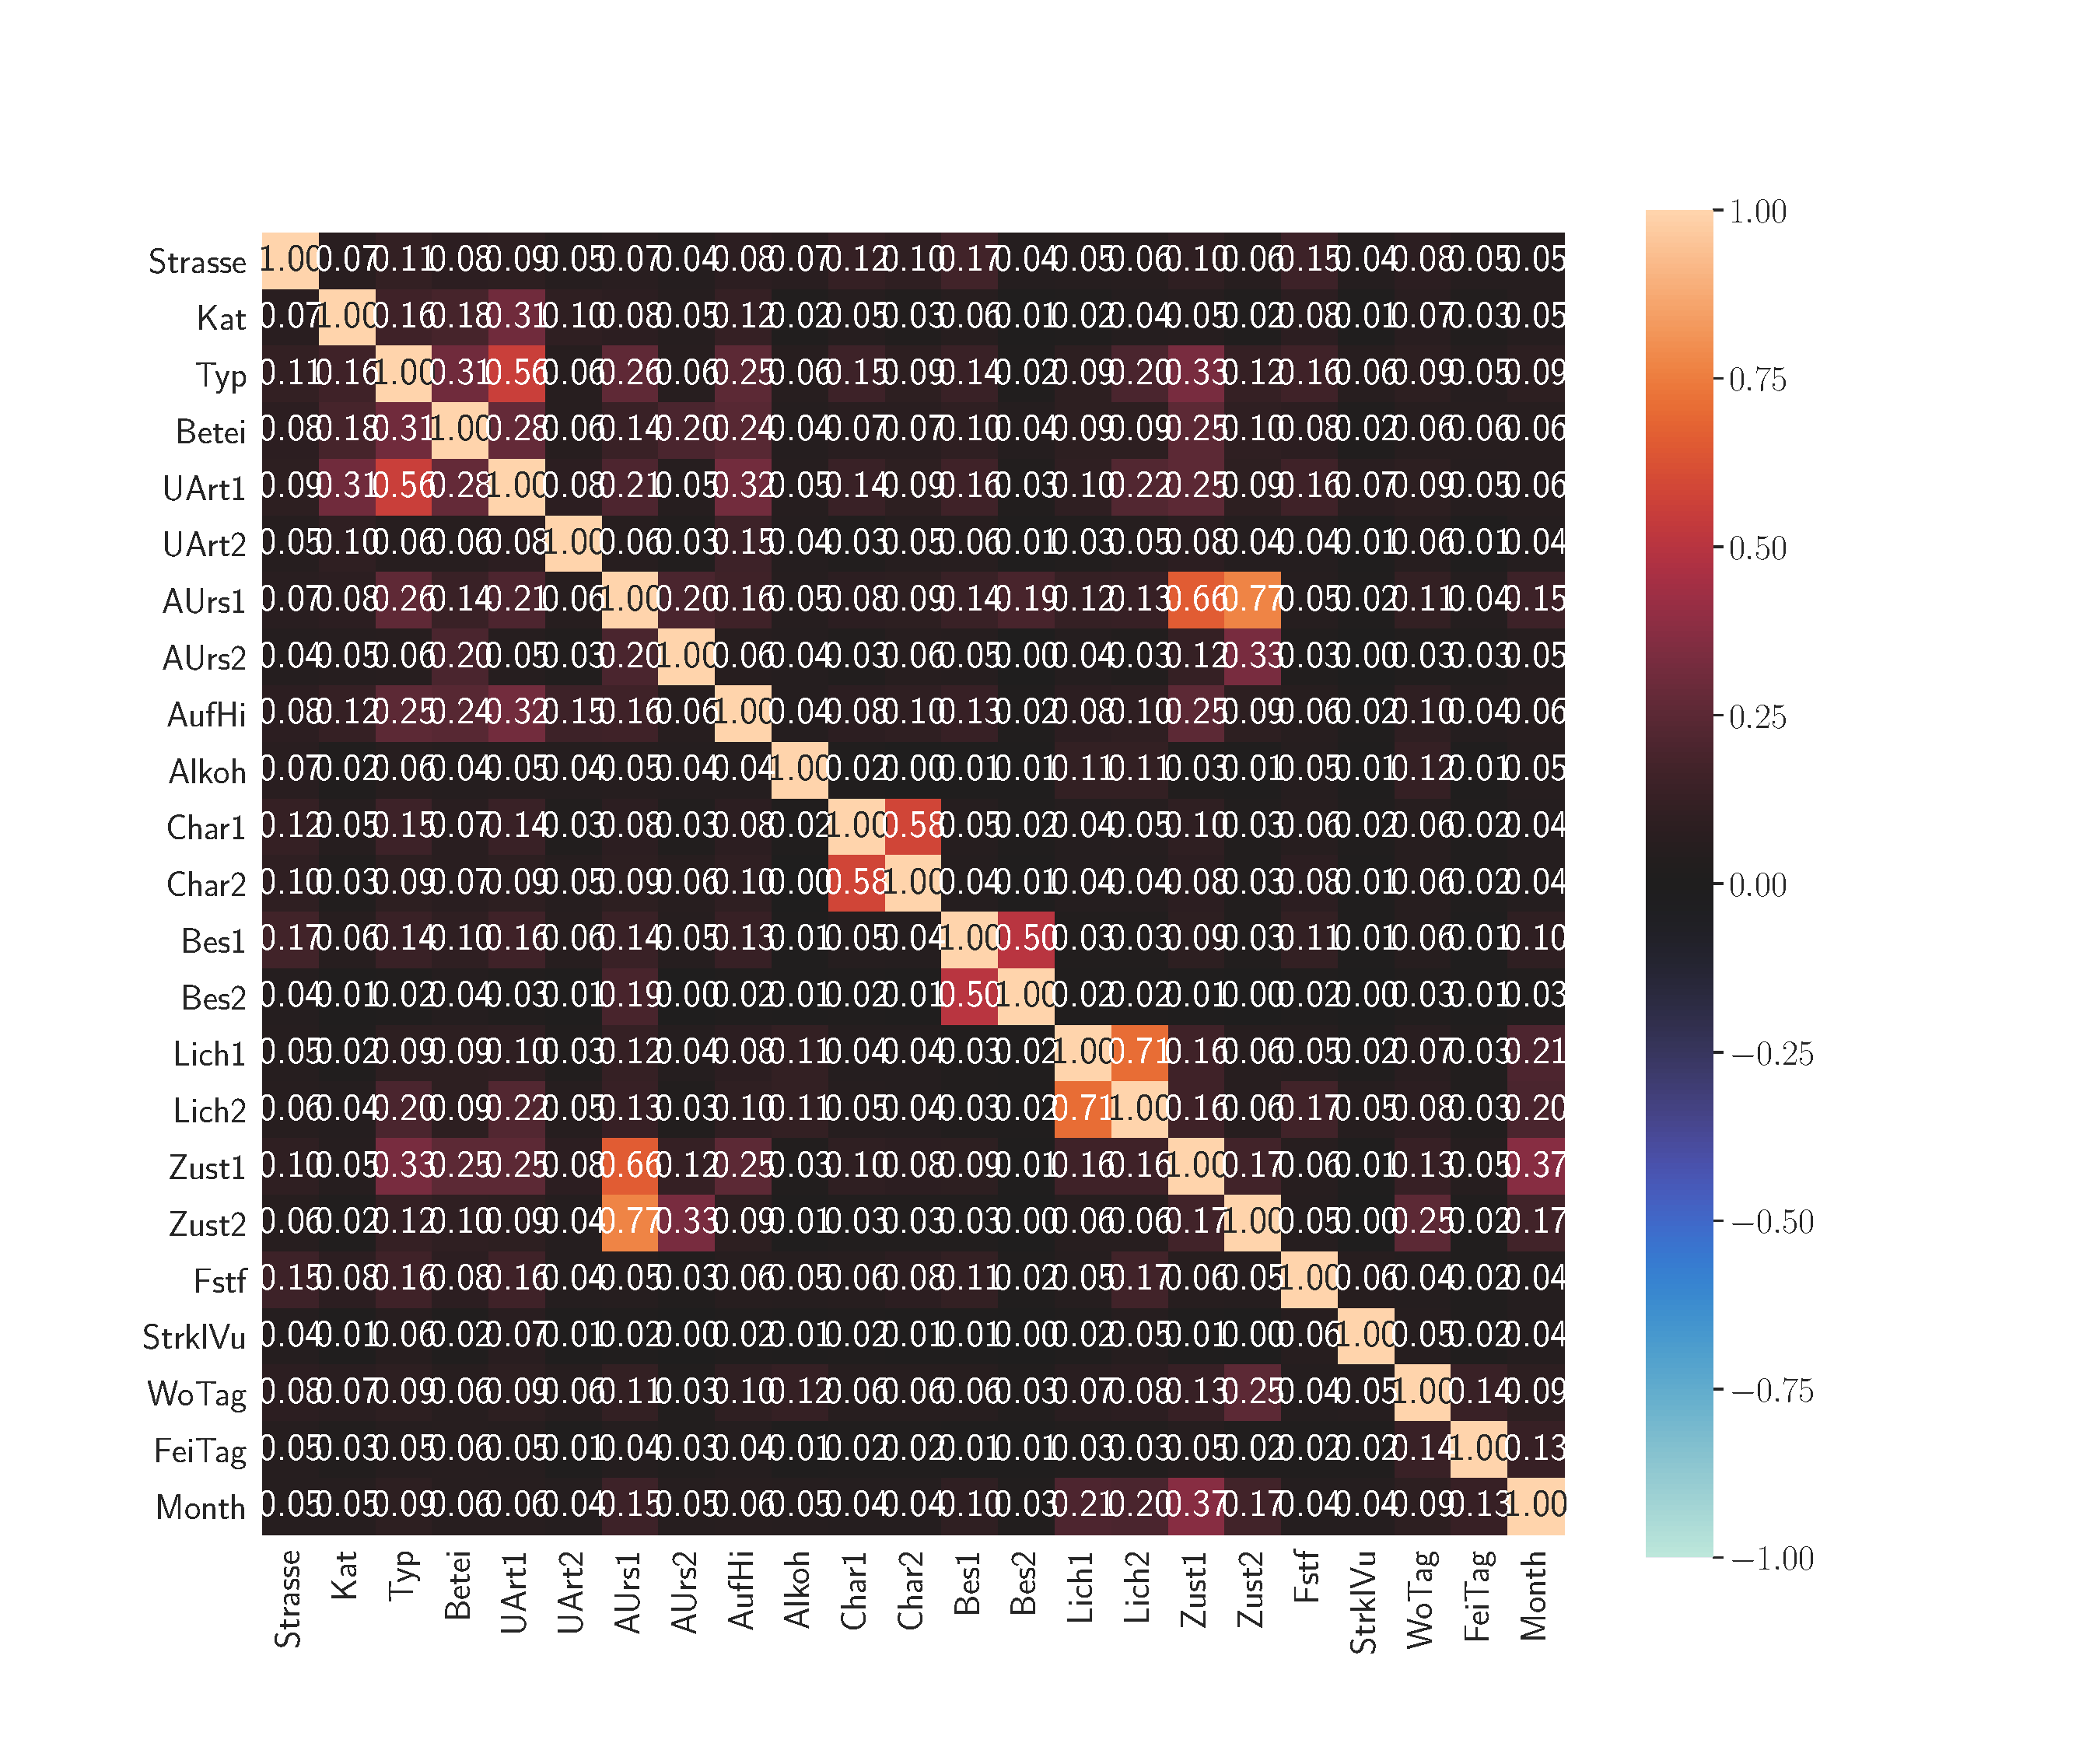
\includegraphics[scale=0.4, trim=4cm 6cm 0cm 6cm]{CorrAnalysis/data/BAYSIS/01_dataset/plots/baysis_dataset_corr_cramers}
% 	\caption{Correlation matrix for BAYSIS dataset, calculated with Cramer's $V$}
% 	\label{img:correlation_matrix_dataset_cramers}
% \end{figure}
% \restoregeometry
% \pagestyle{headings}
% To check for dependent variables which need to be considered in a correlation analysis, the correlation matrix for all relevant parameters in the BAYSIS dataset is calculated for Cramer's $V$. Cramer's $V$ reveals several strong relationships, which are 'Typ'-'UArt1'. 'AUrs1'-'Zust1', 'AUrs1'-'Zust2' and some  trivial relations of 'Char1'-'Char2', 'Bes1'-'Bes2', 'Lich1'-'Lich2'. The results of Theil's $U$ confirms the relationships identified by Cramer's $V$ with a moderate effect size and show the association of 'Aufhi'-'UArt' with a strong effect size. 

% \autoref{tab:baysis_variables} show all categorized parameters, relevant for the correlation analysis, with variable group, type and the format of the containing data. 
% \begin{table}[ht]
% 	\centering
% 	\small
% 	\begin{tabular}{c|c|c|c}
% 		\toprule
% 		\textbf{Variable} 	& \textbf{Group} 	& \textbf{Type} & \textbf{Format} \\
% 		\midrule
% 		Kat  		& categorical 	& ordinal 	& numeric\\
% 		\midrule
% 		Typ 		& categorical 	& nominal	& numeric\\
% 		\midrule
% 		Beteil 		& categorical 	& ordinal	& numeric\\
% 		\midrule
% 		UArt 		& categorical 	& nominal	& numeric\\
% 		\midrule
% 		AUrs 		& categorical 	& nominal	& numeric\\
% 		\midrule
% 		AufHi 		& categorical 	& nominal	& numeric\\
% 		\midrule
% 		Alkoh 		& categorical 	& dichotomous	& numeric\\
% 		\midrule
% 		Char 		& categorical 	& nominal	& numeric\\
% 		\midrule
% 		Bes 		& categorical 	& nominal	& numeric\\
% 		\midrule
% 		Lich 		& categorical 	& ordinal	& numeric\\
% 		\midrule
% 		Zust 		& categorical 	& ordinal	& numeric\\
% 		\midrule
% 		Fstf 		& categorical 	& nominal	& mixed\\
% 		\midrule
% 		WoTag 		& categorical 	& nominal	& text\\
% 		\midrule
% 		FeiTag 		& categorical 	& dichotomous	& numeric\\
% 		\bottomrule
% 	\end{tabular}
% 	\caption{Variable types of \acrshort{baysis} dataset}
% 	\label{tab:baysis_variables}
% \end{table}

The designed evaluation tool, utilizes a PostgreSQL database for its data storage. Therefore the BAYSIS data in form of \acrfull{csv} needs to processed and converted into SQL data entities. Also, the data entities for each accident need to be uniform and comparable with our street network and other entities like roadworks, which makes it necessary to process and map the accidents onto our street network. After the necessary processing and import into the database, 7971 re cords end up being converted and persisted, which equivalent to 77,6\% of the total number of accidents. This 22,4\% of data loss is due to the conversion of from the BAYSIS geo-system to the HERE network, which tries to find a corresponding street network location to the legacy location of the BAYSIS dataset. If it is not able to locate the position of the BYSIS dataset on our street network, the record is discarded.s

\section{Roadwork Data (ArbIS)}
\label{dataset_arbis}

The \acrfull{arbis}, as described in \autoref{dataset_arbis}, is a collection service of all roadworks or maintenance which is planned, ongoing or finished on the Bavarian street network. The dataset for 2019 contains close to 650.000 data-points, which each describe the temporal and spatial extend, road name and number of closed lanes of a roadwork fragment. This fragmentation of events makes is rather hard to statically analyze this dataset since each roadwork is spitted into any number of fragments are only linked by a roadwork identifier. Therefore the analysis of the dataset in this section is rather basic. The import processing works similarly to the \acrshort{baysis} data in \autoref{dataset_baysis} and produces 282.839 roadwork events in the database after the aggregation of fragments. 

With the 4500 long term and more than 40.000 short term building sites on German highways per year \parencite{LAPID2018,Stmi2020}, road construction makes up for the majority of traffic obstructions in the summer months. During the colder month, in which many kinds of construction projects are not possible, snow clearings or long-term constructions are the main obstacles. That also means that the number and type of roadworks varies during the course of a year \parencite{Stmi2020}. 

\begin{figure}[ht]
	\centering
	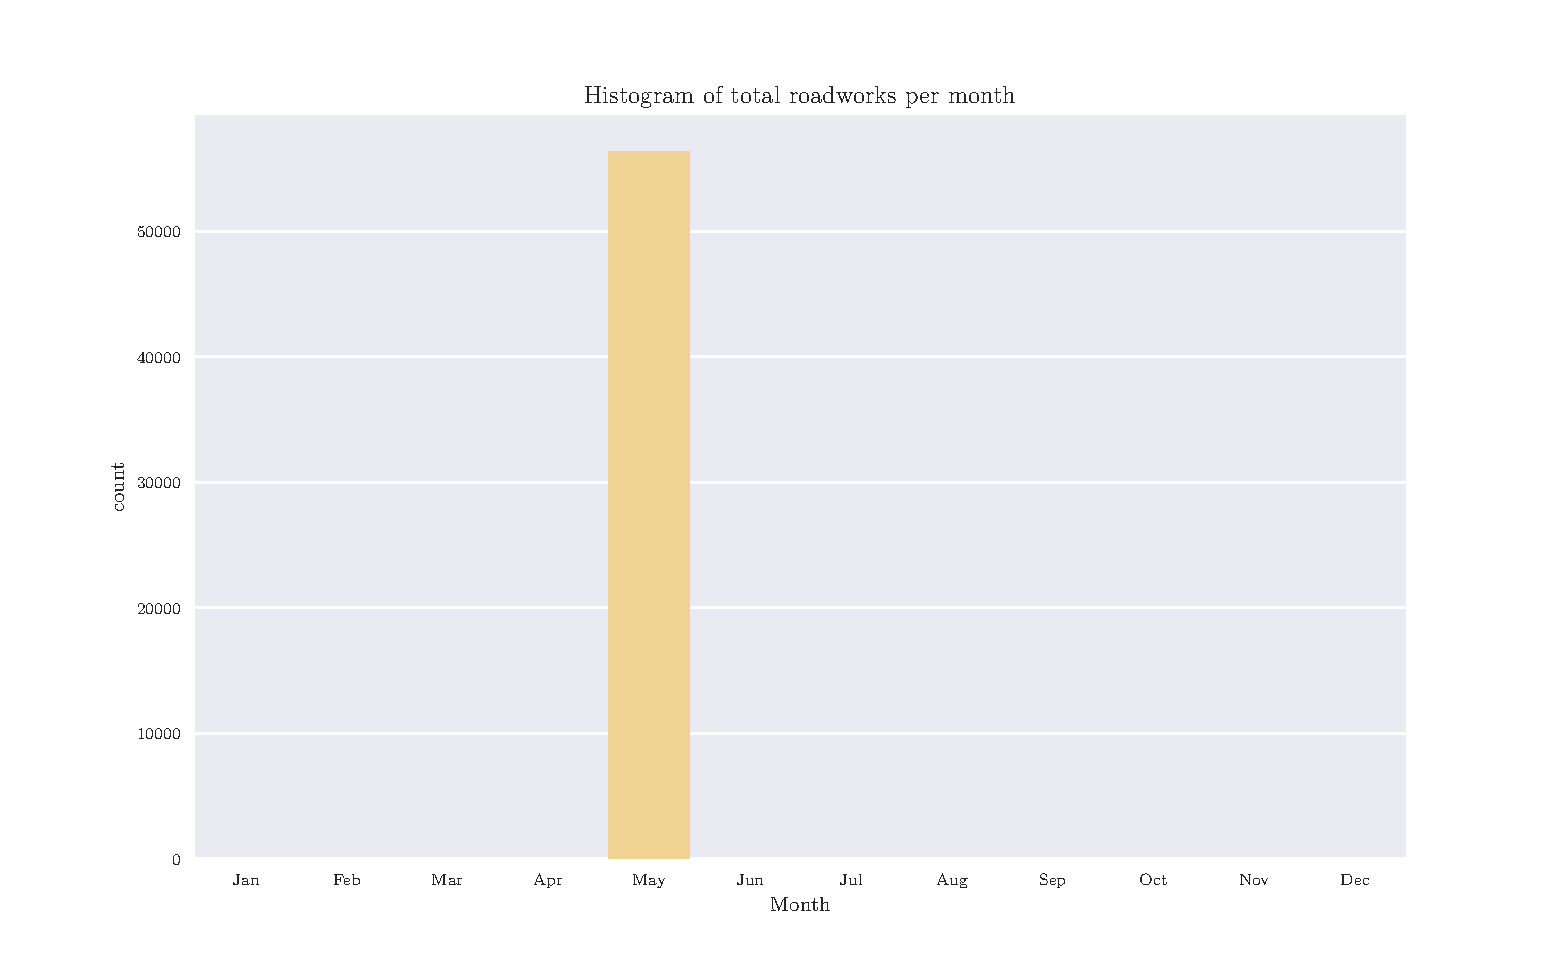
\includegraphics[width=0.7\textwidth]{../CorrAnalysis/data/ArbIS/01_dataset/plots/arbis_dataset_hist_month}
	\caption{Monthly distribution of roadwork fraction counts}
	\label{img:arbis_dataset_dist_month}
\end{figure}

The monthly distribution of roadworks in the year 2019 in figure \autoref{img:arbis_dataset_dist_month} supports this statement, since the winter months of January, February and December tend to have less roadwork that others. The month of July has the most roadworks. Similar to the BAYSIS data the road \textit{A3} and \text{A9} have the highest numbers of roadworks (shown in figure \autoref{img:arbis_dataset_dist_highway}).

\begin{figure}[ht]
	\centering
	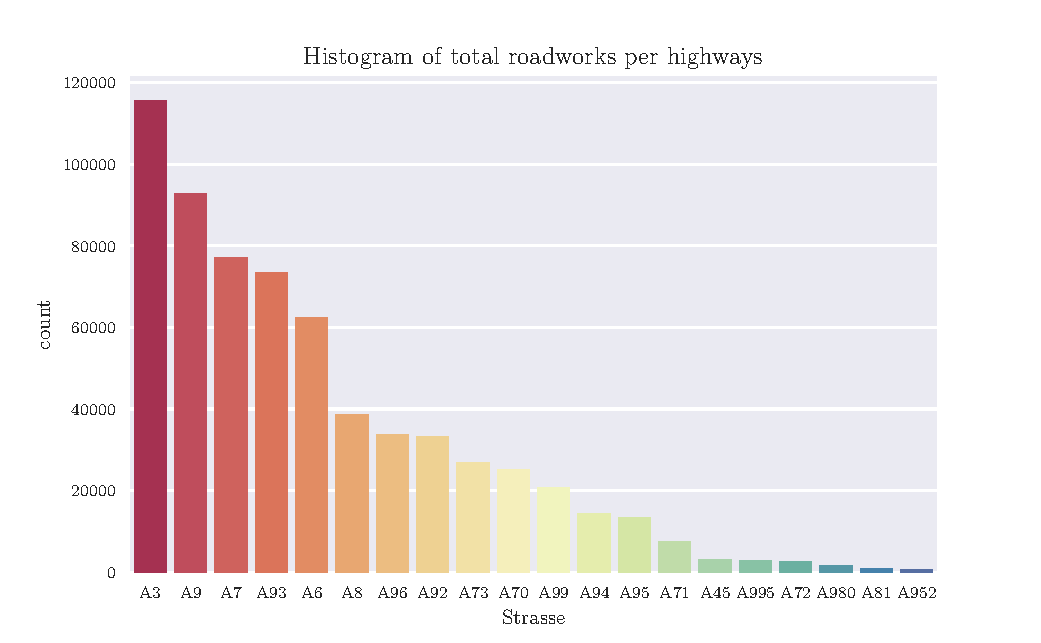
\includegraphics[width=0.7\textwidth]{../CorrAnalysis/data/ArbIS/01_dataset/plots/arbis_dataset_hist_highway}
	\caption{Distribution of roadwork fraction counts, by road}
	\label{img:arbis_dataset_dist_highway}
\end{figure}

\pagebreak

\paragraph{AnzGesperrtFs} refers to the number of closed lanes for the time of the incident. The distribution shows that two states of zero and one block lane hold nearly 100\,\%. Since the variable can be ordered by the number of lane, it is of ordinal type.
\todo{Descriptives}
% \begin{figure}[ht]
% 	\centering
% 	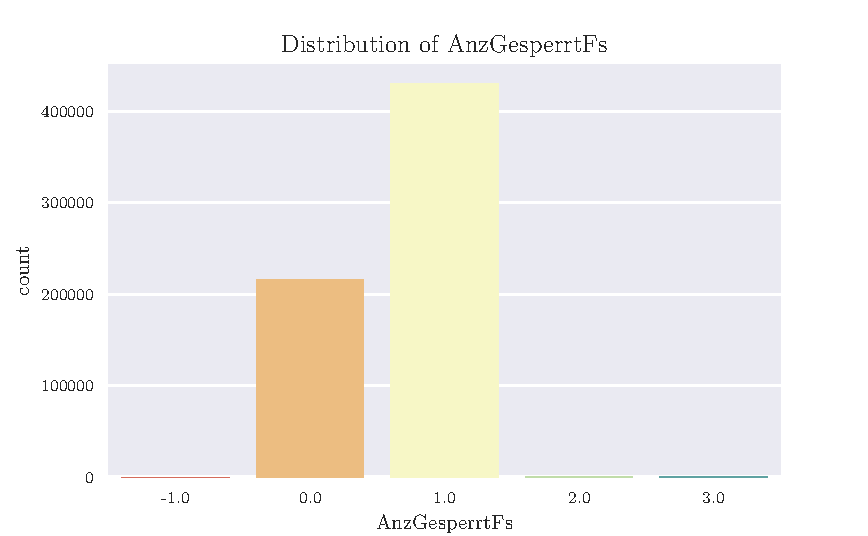
\includegraphics[width=0.7\textwidth]{../CorrAnalysis/data/ArbIS/01_dataset/plots/arbis_dataset_count_AnzGesperrtFs}
% 	\caption{Distribution of roadwork fraction counts, by road}
% 	\label{img:arbis_dataset_count_AnzGesperrtFs}
% \end{figure}

\paragraph{Einzug} describes the shift of the road way due to physical changes, measured in number of lanes. It ranges from one to five lanes, where one, two and five are equally frequent. 
\todo{Descriptives}
% \begin{figure}[ht]
% 	\centering
% 	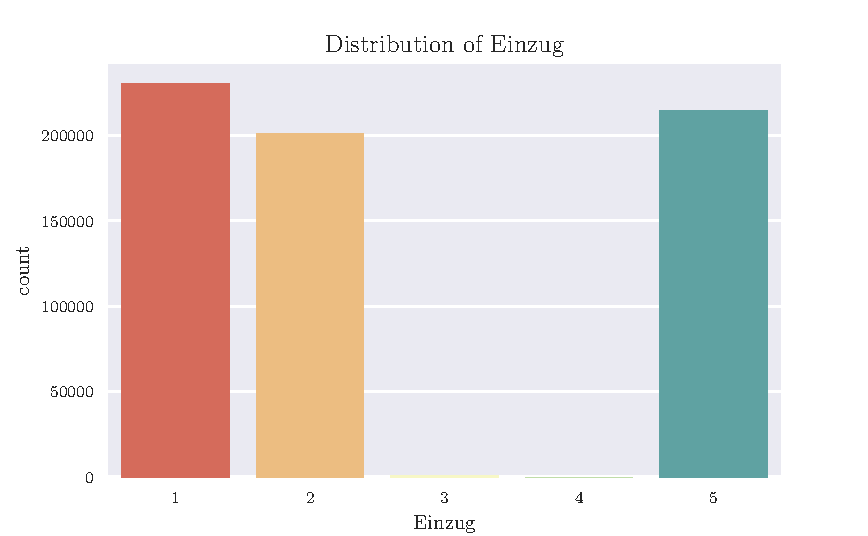
\includegraphics[width=0.7\textwidth]{../CorrAnalysis/data/ArbIS/01_dataset/plots/arbis_dataset_count_Einzug}
% 	\caption{Distribution of roadwork fraction counts, by road}
% 	\label{img:arbis_dataset_count_Einzug}
% \end{figure}

\paragraph{Length} is calculated from the two dataset parameters \textit{VonKilometer} and \textit{BisKilometer}, since it is not part of the original ArbIS dataset. 
\todo{Descriptives}

\paragraph{Duration} is calculated from the two dataset parameters \textit{Von} and \textit{Bis}, since it is not part of the original ArbIS dataset.
\todo{Descriptives}

%\autoref{table:baysis_variables} show all categorized parameters, relevant for the correlation analysis, with variable group, type and the format of the containing data.	
% \begin{table}[ht]
% 	\centering
% 	\begin{tabular}{c|c|c|c}
% 		\toprule
% 		\textbf{Variable} 	& \textbf{Group} 	& \textbf{Type} 		& \textbf{Format} \\
% 		\midrule
% 		AnzGesperrtFs  	& categorical 	& ordinal 	& numeric\\
% 		\midrule
% 		Einzug  		& categorical 	& ordinal 	& numeric\\
% 		\midrule
% 		Length  		& continuous 	& interval 	& numeric\\
% 		\midrule
% 		Duration  		& continuous 	& interval 	& numeric\\
% 		\bottomrule
% 	\end{tabular}
% 	\caption{Variable types of \acrshort{baysis} dataset}
% 	\label{table:arbis_variables}
% \end{table}
